\section{AHTR One-Third Assembly Optimization Results Discussion}
\label{sec:assem-discussion}
Chapter \ref{chap:ahtr-plank-opt-results} characterized the \gls{AHTR} plank model's 
driving factors for each reactor optimization objective and their relationship with 
one another. 
This section utilizes the previous \gls{AHTR} plank characterizations and conduct 
a deep-dive to verify if the same reactor optimization objective driving factors apply 
to the \gls{AHTR} one-third assembly model. 
I also analyze how their combined effects result in the optimal reactor models found by 
the multi-objective optimization simulations. 

\subsection{Discussion: Minimize $PF_{total}$ Objective}
\label{sec:assem-discussion-pf}
\paragraph{Simulation a-1a}
In Section \ref{sec:assem-1-obj-pf}'s simulation a-1a, I conducted a single-objective 
optimization simulation to minimize the one-third assembly's total fuel packing fraction 
($PF_{total}$) by varying $PF_{total}$ and TRISO distribution. 
In simulation a-1a, \gls{ROLLO} found that an \gls{AHTR} one-third assembly model with 
the most-minimized $PF_{total}$ has $PF_{total}= 0.0559$ and an oscillating TRISO distribution 
along the x-axis (Figure \ref{fig:assem-obj-1-pf}).

Section \ref{sec:plank-discussion-pf} concluded that for the \gls{AHTR} plank model, 
the minimize $PF_{total}$ objective is driven by maximizing the total fission reaction 
rates. 
I ran a simulation for constant $PF_{total} = 0.0559$ TRISO distribution and compared its 
fission reaction rate with the oscillating TRISO distribution that most-minimized $PF_{total}$. 
Figure \ref{fig:assem-0.0559-comparison} shows the TRISO distributions for the two compared 
simulations: Figure \ref{fig:assem-obj-1-pf}'s most-minimized $PF_{total}$ 
and the constant $PF_{total} = 0.0559$. 
\begin{figure}[htbp!]
    \centering
    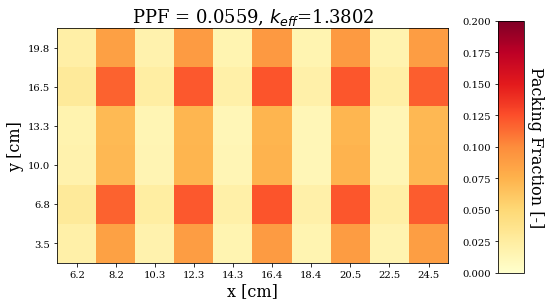
\includegraphics[width=0.49\linewidth]{assem-0.0559-most-minimized.png} 
    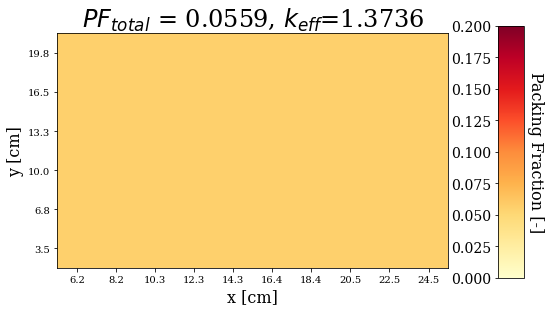
\includegraphics[width=0.49\linewidth]{assem-0.0559-flat.png} 
    \caption{Simulation a-1a's most-minimized $PF_{total}$ TRISO distribution 
    (oscillating TRISO distribution) from Figure \ref{fig:assem-obj-1-pf} (left) and the 
    constant $PF_{total} = 0.0559$ TRISO distribution (right).}
    \label{fig:assem-0.0559-comparison}
\end{figure}
The reactor model with the most-minimized $PF_{total}$ has $k_{eff}=1.3802$ and 
the reactor model with constant TRISO distribution has $k_{eff}=1.3736$.

Table \ref{tab:a-1a-fission-comparison} compares the total fission reaction rate 
(OpenMC's \texttt{fission} tally) between the most-minimized $PF_{total}$ TRISO 
distribution and a constant $PF_{total} = 0.0559$ TRISO distribution (both shown in 
Figure \ref{fig:assem-0.0559-comparison}).
\begin{table}[htbp!]
    \centering
    \onehalfspacing
    \caption{Total fission reaction rate comparison between simulation a-1a's 
    most-minimized $PF_{total}$ TRISO distribution and a constant $PF_{total} = 0.0559$ 
    TRISO distribution.}
	\label{tab:a-1a-fission-comparison}
    \footnotesize
    \begin{tabular}{p{1.5cm}lp{3.7cm}p{4cm}p{2.5cm}}
    \hline
    \textbf{Energy Group} & 
    \textbf{$\%$ of Total} &
    \textbf{Most-minimized $PF_{total}$ Fission \newline [reactions/src]} & 
    \textbf{Flat $PF_{total}$ Fission [reactions/src]} & 
    \textbf{$\%$ Fission \newline Difference}\\
    \hline 
    1 & 00.28 & 0.001659 & 0.001626 & \Plus2.01 \\
    2 & 01.56 & 0.008861 & 0.008842 & \Plus0.21 \\
    3 & 01.51 & 0.008545 & 0.008525 & \Plus0.23 \\
    4 & 96.63 & 0.548134 & 0.544651 & \Plus0.63 \\
    \hline
    \end{tabular}
\end{table}
$96.63\%$ of fission reactions occur in energy group 4. 
In energy group 4, the most-minimized $PF_{total}$ TRISO distribution has $0.63\%$ higher  
\texttt{fission} (total fission reaction rate) than the constant 
$PF_{total} = 0.0559$ TRISO distribution, explaining why the oscillating TRISO 
distribution enabled a 650pcm higher $k_{eff}$ for the same $PF_{total}$ compared to the 
constant TRISO distribution. 

\paragraph{Simulation a-1d}
In Section \ref{sec:assem-1-obj-pf}'s simulation a-1d, I conducted a single-objective 
optimization simulation to minimize total fuel packing fraction ($PF_{total}$) by 
varying $PF_{total}$ and coolant channel shape. 
In simulation a-1d, \gls{ROLLO} found that there is no correlation 
between $PF_{total}$ and coolant channel shape (demonstrated in Figure 
\ref{fig:a-1d}). 

\paragraph{Summary}
I verified that the minimize $PF_{total}$ objective for the \gls{AHTR} one-third assembly 
model is also driven by maximizing the total fission reaction rates. 
The minimize $PF_{total}$ objective has correlations with the following input parameters: 
$PF_{total}$ and TRISO packing fraction distribution. 
The objective has no correlation with coolant channel shape input parameter. 

\subsection{Discussion: Minimize $T_{max}$ Objective}
\label{sec:assem-discussion-temp}

\paragraph{Simulation a-1b}
In Section \ref{sec:assem-1-obj-temp}'s simulation a-1b, I conducted a single-objective 
optimization simulation to minimize the one-third assembly's maximum temperature 
($T_{max}$) by varying TRISO distribution. 
In simulation a-1b, \gls{ROLLO} found that an \gls{AHTR} one-third assembly model with 
a mostly flat TRISO distribution most-minimized $T_{max}$ 
(Figure \ref{fig:assem-obj-1-temp-final}).

\paragraph{Simulation a-1e}
In Section \ref{sec:assem-1-obj-temp}'s simulation a-1e, I conducted a single-objective 
optimization simulation to minimize the one-third assembly's maximum temperature 
($T_{max}$) by varying coolant channel shape. 
In simulation a-1e, \gls{ROLLO} found that there is a negative linear correlation 
between the plank's $T_{max}$ and $r_1$ and $r_5$, but no correlation with 
$r_2$, $r_3$, and $r_4$, shown in Figure \ref{fig:a-1e}. 
% TODO: explain that temperature peaks in the outer planks for this distribution. 
% prove that for a different TRISO distribtion, r2, r3, r4 are correlated to Tmax. 

\paragraph{Summary}


\subsection{Discussion: Minimize $PPF_{fuel}$ Objective}
\label{sec:assem-discussion-ppf}
\paragraph{Simulation a-1c}
In Section \ref{sec:assem-1-obj-ppf}'s simulation a-1c, I conducted a single-objective 
optimization simulation to minimize fuel-normalized power peaking factor ($PPF_{fuel}$) 
by varying TRISO distribution. 
In simulation a-1c, \gls{ROLLO} found that for $PF_{total}$ = 0.06, the reactor model 
with the most-minimized $PPF_{fuel}$ has a $PPF_{fuel} = 1.0872$ and an oscillating 
TRISO distribution along the x-axis with peaks on the x-axis at the 7.8cm, 
15.9cm, and 22.0cm; and each row has a packing fraction variation of $\sim0.05$.

Section \ref{sec:assem-discussion-pf} concluded that for the \gls{AHTR} plank 
model, the minimize $PPF_{fuel}$ objective is driven by flattening thermal 
(Group 4) flux distribution. 
I compare the flux distributions for the most-minimized $PPF_{fuel}$ reactor model  
($PPF_{fuel} = 1.0872$) and the reactor model in simulation a-1c's final generation
with the highest $PPF_{fuel} = 1.2431$. 
Figure \ref{fig:a-1c-ppf-triso-comparison} shows the TRISO distributions for the 
compared reactor models. 
\begin{figure}[htbp!]
    \centering
    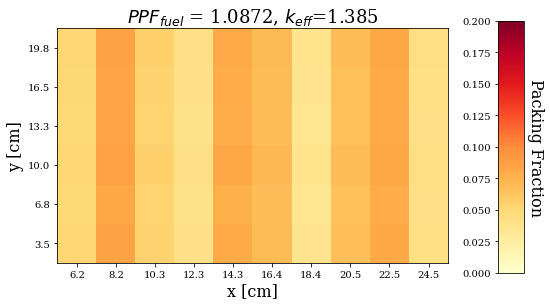
\includegraphics[width=0.49\linewidth]{a-1c-ppf-triso-comparison-most-minimized.png} 
    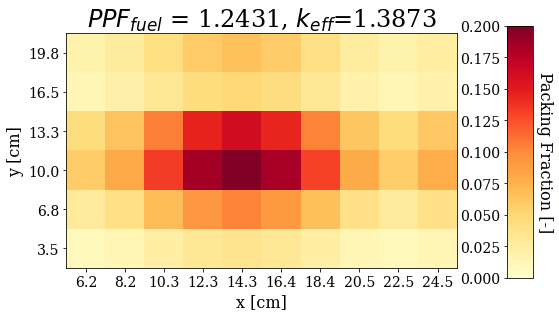
\includegraphics[width=0.49\linewidth]{a-1c-ppf-triso-comparison-least-minimized.png} 
    \caption{Simulation a-1c's most-minimized $PPF_{fuel}$ TRISO distribution 
    from Figure \ref{fig:assem-obj-1-ppf} (left) and the highest $PPF_{fuel}$ TRISO distribution (right).}
    \label{fig:a-1c-ppf-triso-comparison}
\end{figure}

Figure \ref{fig:a-1c-flux-comparison} compares the flux distributions between 
simulation a-1c's most-minimized $PPF_{fuel}$ TRISO distribution and highest 
$PPF_{fuel}$ TRISO distribution (both distributions shown in Figure 
\ref{fig:a-1c-ppf-triso-comparison}). 
\begin{figure}[htbp!]
    \centering
    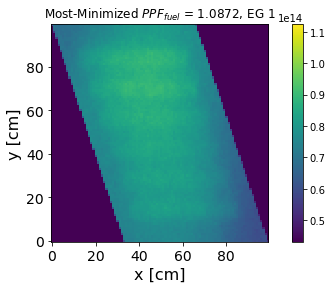
\includegraphics[width=0.35\linewidth]{flux-comparison-a-1c-most-minimized-grp1.png} 
    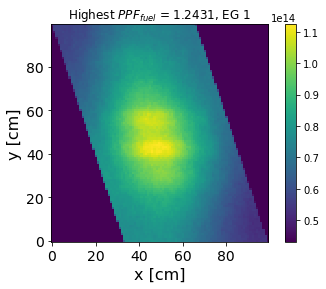
\includegraphics[width=0.35\linewidth]{flux-comparison-a-1c-least-minimized-grp1.png} 
    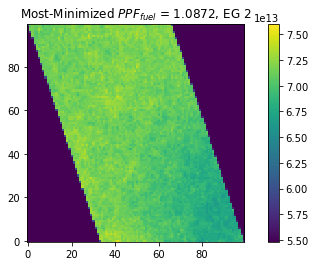
\includegraphics[width=0.35\linewidth]{flux-comparison-a-1c-most-minimized-grp2.png} 
    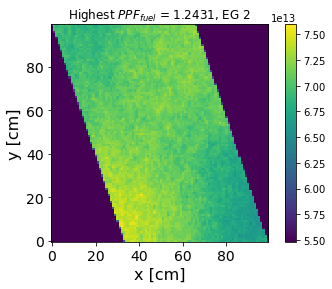
\includegraphics[width=0.35\linewidth]{flux-comparison-a-1c-least-minimized-grp2.png} 
    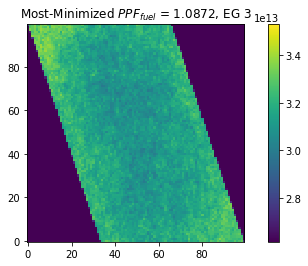
\includegraphics[width=0.35\linewidth]{flux-comparison-a-1c-most-minimized-grp3.png} 
    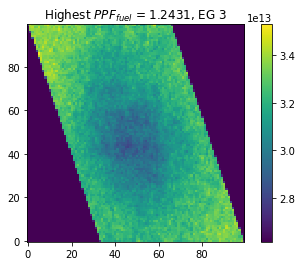
\includegraphics[width=0.35\linewidth]{flux-comparison-a-1c-least-minimized-grp3.png} 
    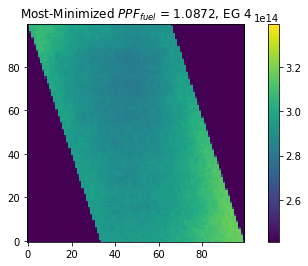
\includegraphics[width=0.35\linewidth]{flux-comparison-a-1c-most-minimized-grp4.png} 
    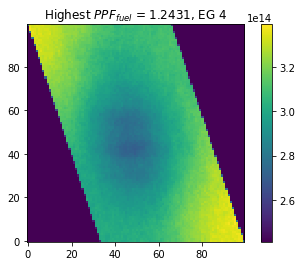
\includegraphics[width=0.35\linewidth]{flux-comparison-a-1c-least-minimized-grp4.png} 
    \caption{AHTR one-third assembly's flux comparison between the two reactor models 
    in Figure \ref{fig:a-1c-ppf-triso-comparison}: simulation a-1c's most-minimized 
    $PPF_{fuel}$ reactor model with $PPF_{fuel} = 1.0872$ and simulation a-1c's reactor 
    model with the highest $PPF_{fuel} = 1.2431$.
    Energy Group 1: E $> 9.1188 \times 10^{-3}$ MeV, 
    Energy Group 2: $2.9023 \times 10^{-5} < E < 9.1188 \times 10^{-3}$ MeV,
    Energy Group 3:  $1.8556 \times 10^{-5} < E < 2.9023 \times 10^{-5}$ MeV,
    Energy Group 4:  $1.0 \times 10^{-12} < E < 1.8554 \times 10^{-6}$ MeV.}
    \label{fig:a-1c-flux-comparison}
\end{figure}

% comment

Table \ref{tab:a-1c-flux-comparison} quantifies the total flux differences per energy group 
between the compared reactor models. 
The flux values were tallied for each energy group within the one-third assembly model 
using a 100 x 100 mesh. 
% describe max and min phi, and the difference calculation. 
\begin{table}[htbp!]
    \centering
    \onehalfspacing
    \caption{Flux value comparison between the two reactor models in Figure 
    \ref{fig:a-1c-ppf-triso-comparison}: simulation a-1c's most-minimized $PPF_{fuel}$ reactor model 
    with $PPF_{fuel} = 1.0872$ and simulation a-1c's reactor model with the highest 
    $PPF_{fuel} = 1.2431$.
    Energy Group 1: E $> 9.1188 \times 10^{-3}$ MeV, 
    Energy Group 2: $2.9023 \times 10^{-5} < E < 9.1188 \times 10^{-3}$ MeV,
    Energy Group 3:  $1.8556 \times 10^{-5} < E < 2.9023 \times 10^{-5}$ MeV,
    Energy Group 4:  $1.0 \times 10^{-12} < E < 1.8554 \times 10^{-6}$ MeV.}
	\label{tab:a-1c-flux-comparison}
    \footnotesize
    \begin{tabular}{lp{4cm}p{3.3cm}p{4cm}}
    \hline
    \textbf{Energy Group} &
    \textbf{$max(\phi)/min(\phi)$ Most-minimized $PPF_{fuel}$ TRISO Distribution} & 
    \textbf{$max(\phi)/min(\phi)$ Highest $PPF_{fuel}$ TRISO Distribution} & 
    \textbf{$\%$ Difference}\\
    \hline 
    1 & 1.825 & 2.608 & \Minus30.00 \\
    2 & 1.341 & 1.386 & \Minus3.18 \\
    3 & 1.302 & 1.334 & \Minus2.43 \\
    4 & 1.319 & 1.331 & \Minus0.85 \\
    \hline
    \end{tabular}
\end{table}

In energy group 4, the most-minimized $PPF_{fuel}$ flux distribution is $0.85\%$ flatter 
than the reactor model with the highest $PPF_{fuel} = 1.2431$ (as shown by Equation 
\ref{eq:flux-prop-ppf}). 
These results verify that similar to the \gls{AHTR} plank model, the \gls{AHTR} one-third 
assembly model's minimize $PPF_{fuel}$ objective is also driven by flattening thermal 
(Group 4) flux distribution. 

\paragraph{Simulation p-1f}
In Section \ref{sec:assem-1-obj-ppf}'s simulation a-1f, I conducted a single-objective 
optimization simulation to minimize fuel-normalized power peaking factor ($PPF_{fuel}$) by 
varying coolant channel shape. 
In simulation a-1f, \gls{ROLLO} found that there is no correlation 
between $PPF_{fuel}$ and coolant channel shape (demonstrated in Figure 
\ref{fig:a-1f}). 

\paragraph{Summary}

\subsection{Discussion: Multi-Objective Optimization}
\label{sec:assem-discussion-multi}

\subsubsection{Simulation a-2a}

\subsubsection{Simulation a-2b}
% compare reactor models 1,3,5's fission reaction rate and thermal flux flattness
In Section \ref{sec:a-2b}'s simulation a-2b, I conducted a two-objective 
optimization simulation to minimize total fuel packing fraction ($PF_{total}$) and 
fuel-normalized power peaking factor ($PPF_{fuel}$) in a one-third assembly model 
by varying TRISO distribution. 
In simulation a-2b, ROLLO found 6 reactor models on the Pareto Front (Figure 
\ref{fig:assem-obj-2-pfppf-pareto}). 

Figure \ref{fig:a-2b-comparison-reactors} shows the TRISO packing fraction distribution 
for 3 reactors models on Figure \ref{fig:assem-obj-2-pfppf-pareto}'s Pareto Front: 
reactor model 1 with most-minimized $PPF_{fuel}$, reactor model 3 with most-minimized 
$PF_{total}$, and reactor model 5 that minimizes both $PF_{total}$ and $PPF_{fuel}$ to an 
equal extent.
\begin{figure}[htbp!]
    \centering
    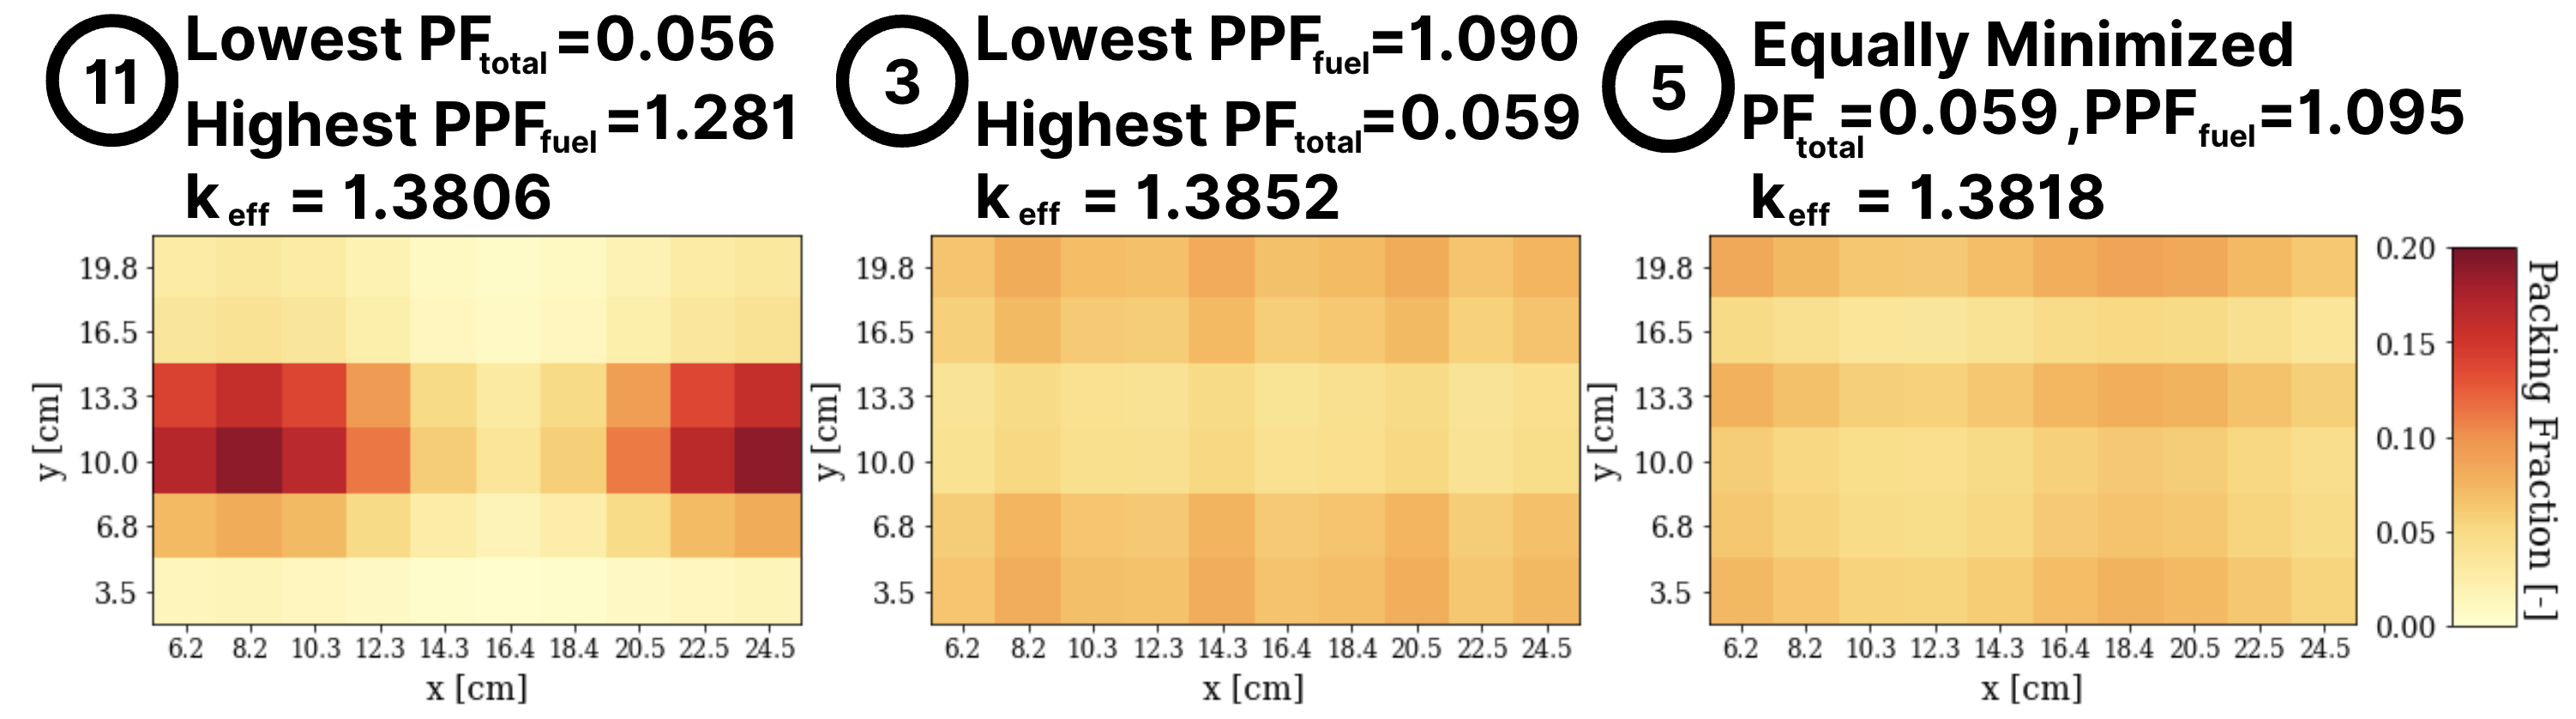
\includegraphics[width=\linewidth]{a-2b-comparison-reactors.png}  
    \caption{TRISO distributions for 3 reactor models on Simulation a-2b's Pareto Front (Figure 
    \ref{fig:assem-obj-2-pfppf-pareto}): reactor model 1 with most-minimized $PPF_{fuel}$ (left), 
    reactor model 3 with most-minimized $PF_{total}$ (middle), and reactor model 5 that 
    minimizes both $PF_{total}$ and $PPF_{fuel}$ to an equal extent (right).}
    \label{fig:a-2b-comparison-reactors}
\end{figure}

Table \ref{tab:a-2b-comparison-reactors} shows the $PF_{total}$, $PPF_{fuel}$, TRISO 
packing fraction distribution variance, total fission reaction rate, and thermal flux 
flatness for the three reactor models. 
\begin{table}[htbp!]
    \centering
    \onehalfspacing
    \caption{$PF_{total}$, $PPF_{fuel}$, TRISO packing fraction distribution variance, 
    total fission reaction rate, and thermal flux flatness for 3 reactor models on Simulation 
    a-2b's Pareto Front (Figure \ref{fig:assem-obj-2-pfppf-pareto}): reactor model 1 with 
    most-minimized $PPF_{fuel}$, reactor model 3 with most-minimized $PF_{total}$, 
    and reactor model 5 that minimizes both $PF_{total}$ and $PPF_{fuel}$ to an equal extent.}
	\label{tab:a-2b-comparison-reactors}
    \footnotesize
    \begin{tabular}{p{3cm}p{1.5cm}p{2.5cm}p{2.5cm}lp{2.5cm}l}
    \hline
    & \textbf{Reactor Model} 
    & \textbf{TRISO distr variance} & \textbf{Fission Reaction Rate} & \textbf{$\%$ Diff}
    & $max(\phi_4)/min(\phi_4)$ & \textbf{$\%$ Diff}\\
    \hline 
    \textbf{Most Minimized Both} & 5 & 0.00044 & 0.5472 & - & 1.2897 &\\
    \textbf{Most Minimized $PF_{total}$} & 3 & 0.00105 & 0.5476 & \Plus0.07 & 1.2949 & \Plus0.40\\
    \textbf{Most Minimized $PPF_{fuel}$} & 1 & 0.00018 & 0.5478 & \Plus0.12 & 1.2851 & \Minus0.35\\
    \hline
    \end{tabular}
\end{table}

The most minimized $PPF_{fuel}$ reactor model (1) has the highest fission reaction rate, 
followed by the most minimized $PF_{fuel}$ reactor model (3), and reactor model 5 that 
minimizes both $PF_{total}$ and $PPF_{fuel}$ to an equal extent.
Reactor model 3 has a higher fission reaction rate compared to reactor model 5 despite having 
a lower $PF_total$.
This is due to reactor model 3's high variance oscillating TRISO distribution, which enables
a higher fission reaction rate, and thus, 240pcm higher $k_{eff}$ for a lower $PF_{total}$
compared to reactor model 5. 

The most minimized $PPF_{fuel}$ reactor model (1) has the flattest thermal flux, followed by 
reactor model 5 that minimizes both $PF_{total}$ and $PPF_{fuel}$ to an equal extent, and 
then the most minimized $PF_{fuel}$ reactor model (3). 
Section xx verified that the \gls{AHTR} one-third assembly model's minimize $PPF_{fuel}$ 
objective is also driven by flattening thermal (Group 4) flux distribution. 
Therefore, reactor model 3 has the flattest thermal flux distribution. 


\subsubsection{Simulation a-2c}

\subsubsection{Simulation a-3a}

\subsubsection{Simulation a-3b}

\subsection{Discussion: Major Takeaways}

\section{Summary}

% talk about p-3b result, what is recommended for the AHTR assembly's geometry. 